\documentclass[english]{beamer}\usepackage[]{graphicx}\usepackage[]{xcolor}
% maxwidth is the original width if it is less than linewidth
% otherwise use linewidth (to make sure the graphics do not exceed the margin)
\makeatletter
\def\maxwidth{ %
  \ifdim\Gin@nat@width>\linewidth
    \linewidth
  \else
    \Gin@nat@width
  \fi
}
\makeatother

\definecolor{fgcolor}{rgb}{0.345, 0.345, 0.345}
\newcommand{\hlnum}[1]{\textcolor[rgb]{0.686,0.059,0.569}{#1}}%
\newcommand{\hlsng}[1]{\textcolor[rgb]{0.192,0.494,0.8}{#1}}%
\newcommand{\hlcom}[1]{\textcolor[rgb]{0.678,0.584,0.686}{\textit{#1}}}%
\newcommand{\hlopt}[1]{\textcolor[rgb]{0,0,0}{#1}}%
\newcommand{\hldef}[1]{\textcolor[rgb]{0.345,0.345,0.345}{#1}}%
\newcommand{\hlkwa}[1]{\textcolor[rgb]{0.161,0.373,0.58}{\textbf{#1}}}%
\newcommand{\hlkwb}[1]{\textcolor[rgb]{0.69,0.353,0.396}{#1}}%
\newcommand{\hlkwc}[1]{\textcolor[rgb]{0.333,0.667,0.333}{#1}}%
\newcommand{\hlkwd}[1]{\textcolor[rgb]{0.737,0.353,0.396}{\textbf{#1}}}%
\let\hlipl\hlkwb

\usepackage{framed}
\makeatletter
\newenvironment{kframe}{%
 \def\at@end@of@kframe{}%
 \ifinner\ifhmode%
  \def\at@end@of@kframe{\end{minipage}}%
  \begin{minipage}{\columnwidth}%
 \fi\fi%
 \def\FrameCommand##1{\hskip\@totalleftmargin \hskip-\fboxsep
 \colorbox{shadecolor}{##1}\hskip-\fboxsep
     % There is no \\@totalrightmargin, so:
     \hskip-\linewidth \hskip-\@totalleftmargin \hskip\columnwidth}%
 \MakeFramed {\advance\hsize-\width
   \@totalleftmargin\z@ \linewidth\hsize
   \@setminipage}}%
 {\par\unskip\endMakeFramed%
 \at@end@of@kframe}
\makeatother

\definecolor{shadecolor}{rgb}{.97, .97, .97}
\definecolor{messagecolor}{rgb}{0, 0, 0}
\definecolor{warningcolor}{rgb}{1, 0, 1}
\definecolor{errorcolor}{rgb}{1, 0, 0}
\newenvironment{knitrout}{}{} % an empty environment to be redefined in TeX

\usepackage{alltt}

%% The most common packages are already included in:
\usetheme{biostat}
%%%%%%%%%%%%%%%%%%%%%%%%%%%%%%%%%%%%%%%%%%%%%%%%%%%%%%%% 

%% Header data: (adjust to your needs:
\def\uzhunit{Master Program in Biostatistics}             %% if (not) needed comment/uncomment
%\def\uzhunitext{STA480}
\title[Recruitment rate stochasticity
at the design stage of a clinical trial, Master Exam]{Frequentists and Bayesian methods to incorporate
recruitment rate stochasticity
at the design stage of a clinical trial}
%% Optional Argument in [Brackets]: Short Title for Footline

%% The following are all optional, simply comment them
\author{Supervision by Malgorzata Roos}
\institute{Biostatistics Master Exam}  %% optional
\subtitle{Pilar Pastor Martínez}
%\date{\today}
%%%%%%%%%%%%%%%%%%%%%%%%%%%%%%%%%%%%%%%%%%%%%%%%%%%%%%%% 




%%%%%%%%%%%%%%%%%%%%%%%%%%%%%%%%%%%%%%%%%%%%%%%%%%%%%%%% 
\IfFileExists{upquote.sty}{\usepackage{upquote}}{}
\begin{document}
\maketitle
%%%%%%%%%%%%%%%%%%%%%%%%%%%%%%%%%%%%%%%%%%%%%%%%%%%%%%%% 
%% Start with slides here: put them between `\begin{frame}` and `\end{frame}`

\begin{frame}{Content}

\begin{itemize}
\item Recruitment and Patient Leakage
\item Methods for Recruited Counts
\item Methods for Waiting Time
\item Exact methods vs MC simulations
\item Conclusions
\item Reproducibility (\href{https://github.com/ppasto/masterthesis}{GitHub})
\end{itemize}

\end{frame}

\begin{frame}{Recruitment and Patient Leakage}

\end{frame}

\begin{frame}{Why recruitment rates?}

According to \cite{carter2004application}
\begin{itemize}
\item Timely recruitment vital to the success of a clinical trial
\item Inadequate number of patients $\rightarrow$ lack of power
\item Recruitment period too long $\rightarrow$ competing treatments
\item Recruitment of patients varies at each stage 
\item Methods applicable to all the stages
\end{itemize}

\end{frame}



\begin{frame}{CONSORT}
\begin{center}
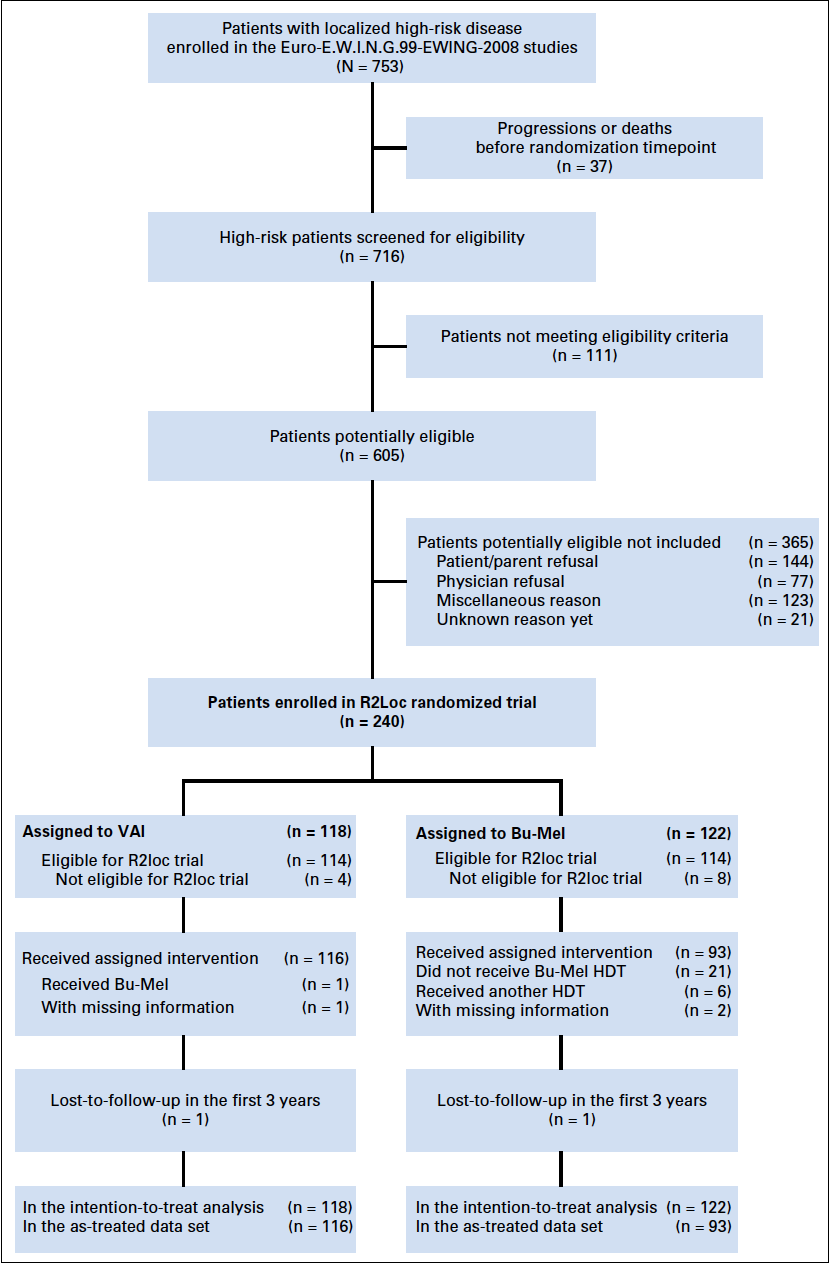
\includegraphics[width=0.4\textwidth]{whelan_flow.png}
\end{center}
\end{frame}

\begin{frame}{Target Population}

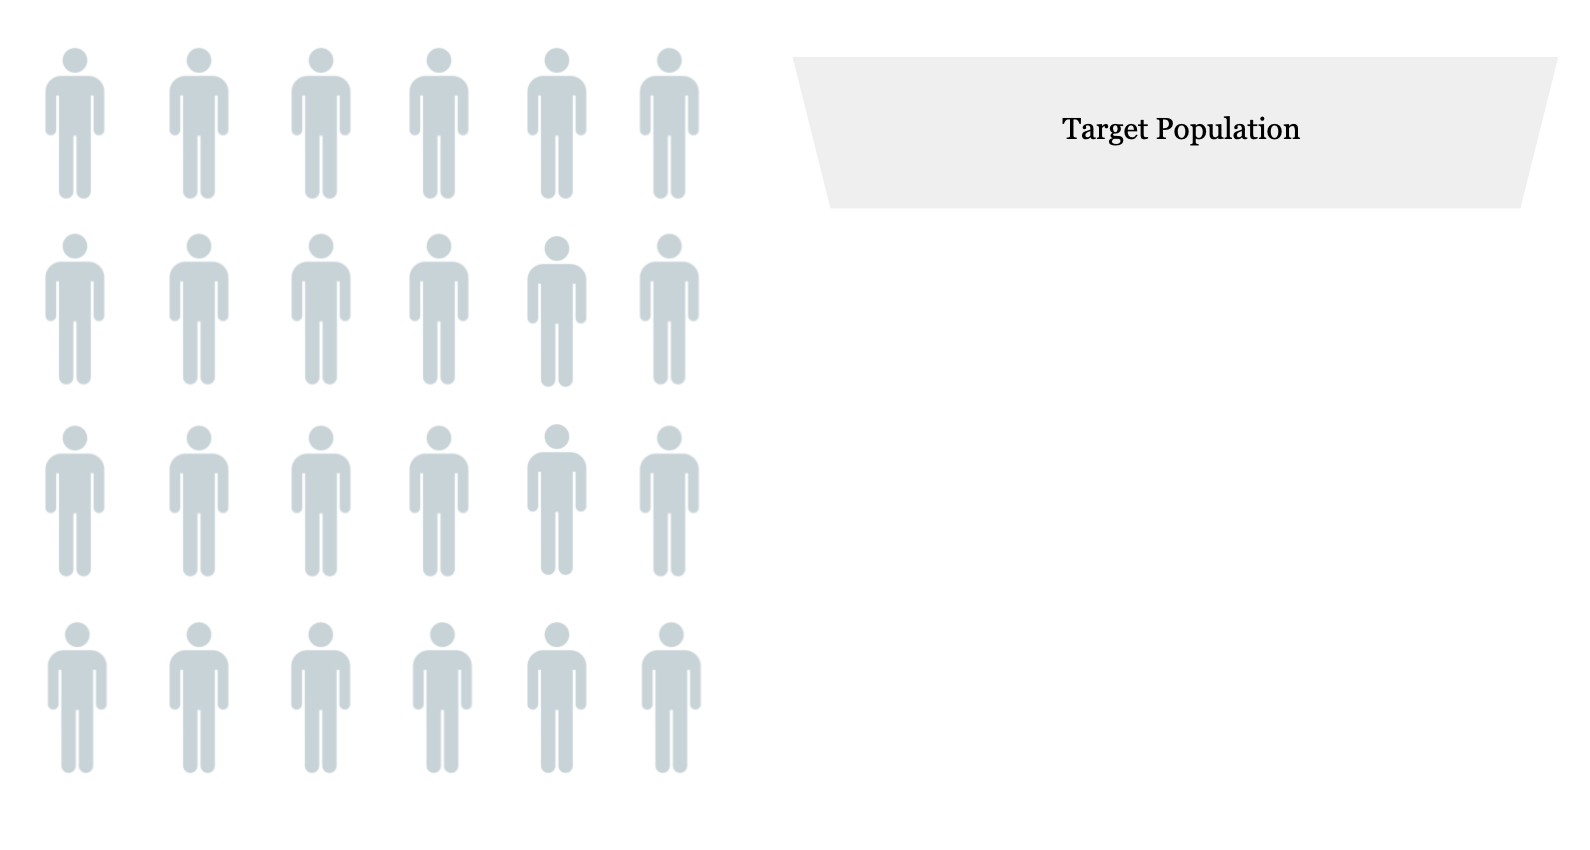
\includegraphics[width=100mm,scale=1]{targetpop.png}

\end{frame}

\begin{frame}{Eligibility}

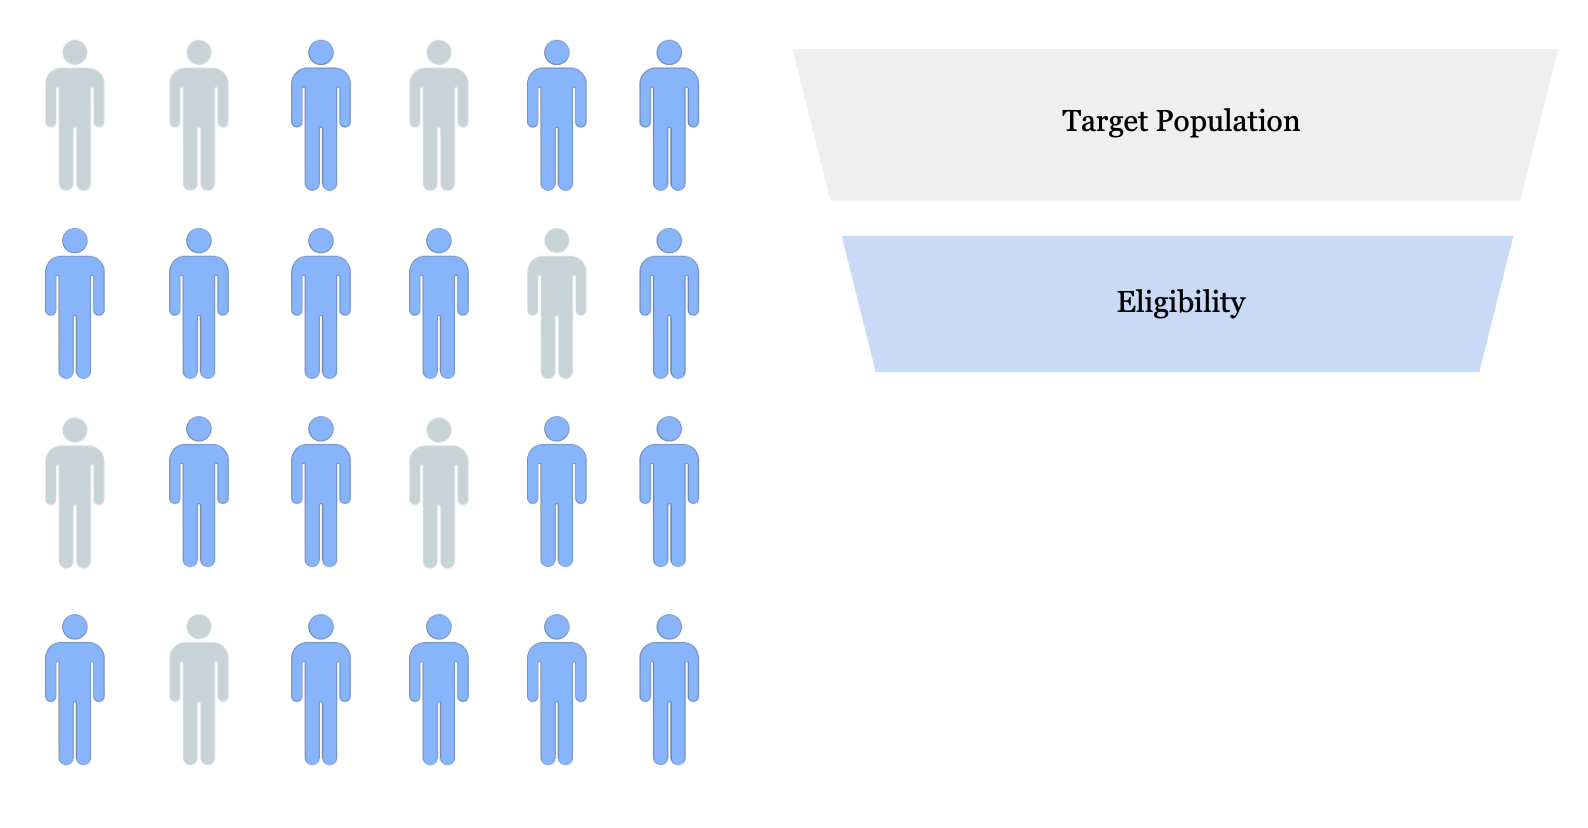
\includegraphics[width=100mm,scale=1]{eligibility.png}

\end{frame}

\begin{frame}{Enrollment}

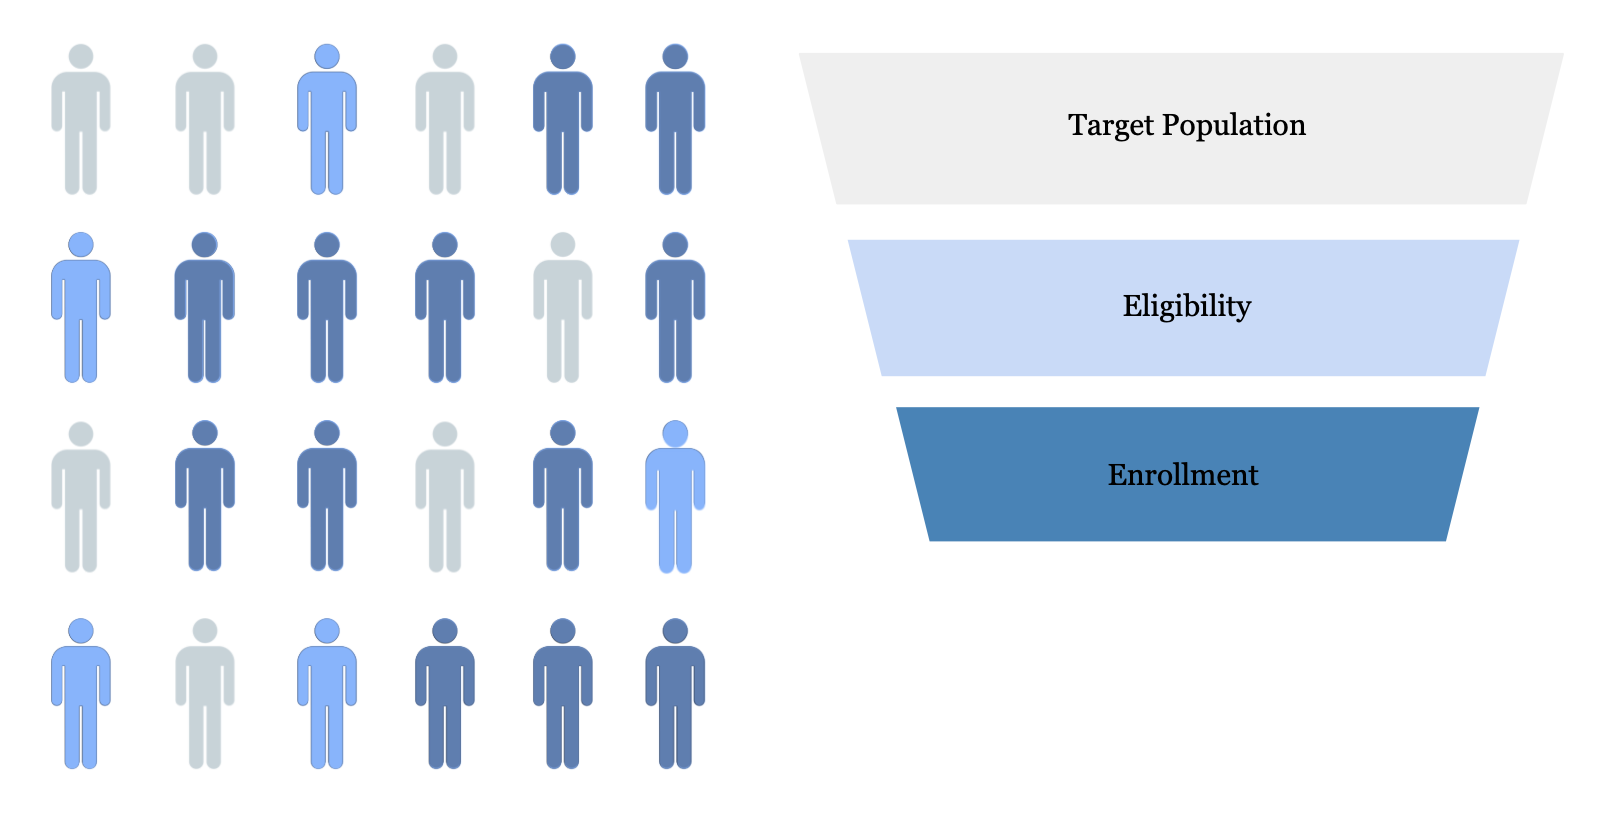
\includegraphics[width=100mm,scale=1]{enrollment.png}


\end{frame}

\begin{frame}{Randomization}

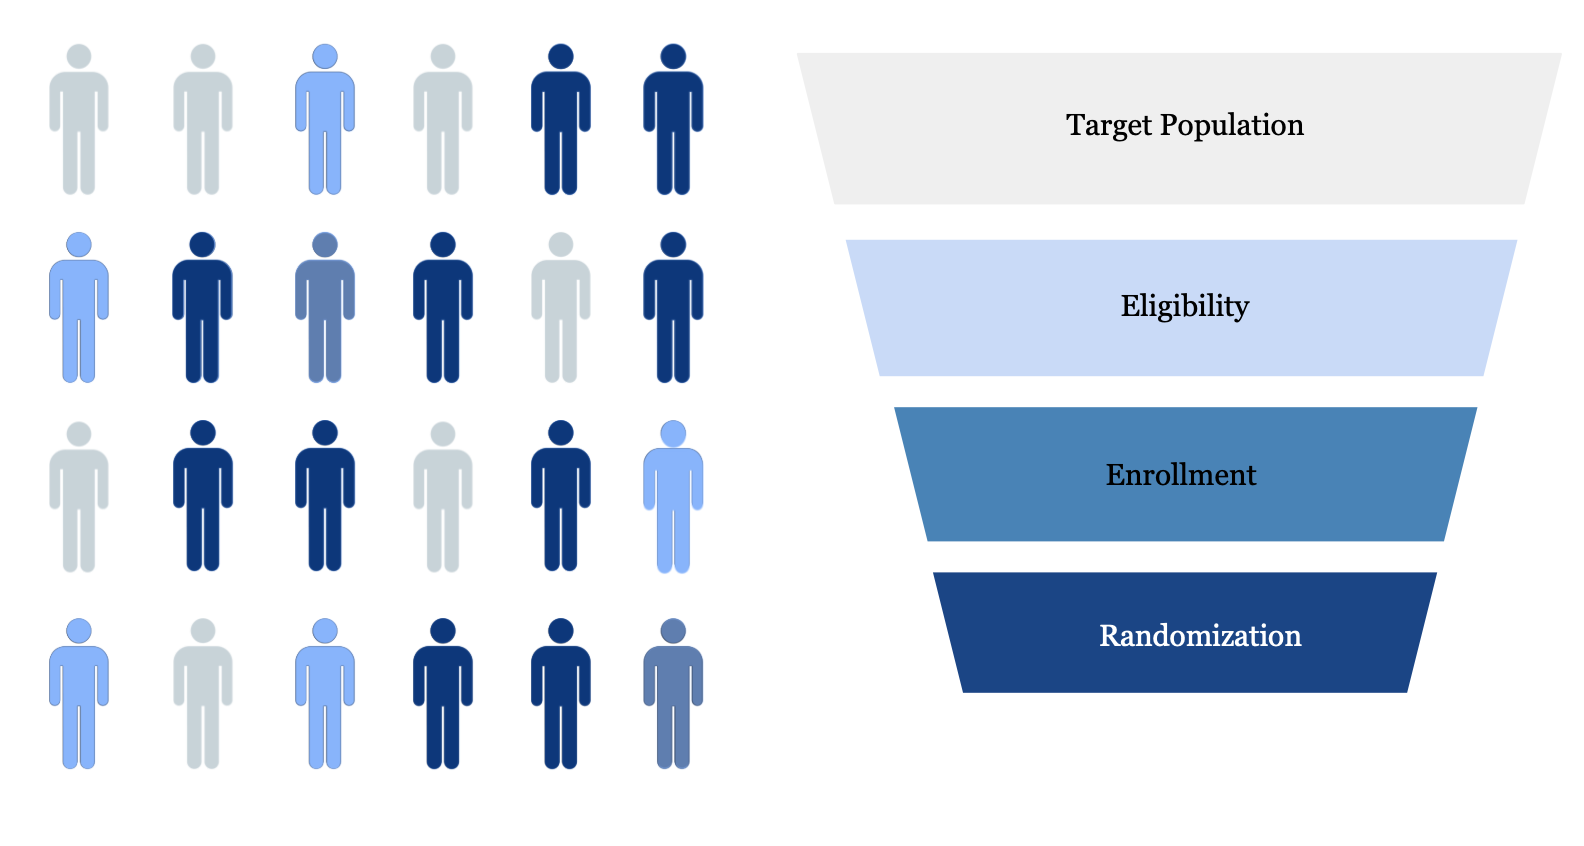
\includegraphics[width=100mm,scale=1]{randomization.png}

\end{frame}

\begin{frame}{Statistical Analysis}

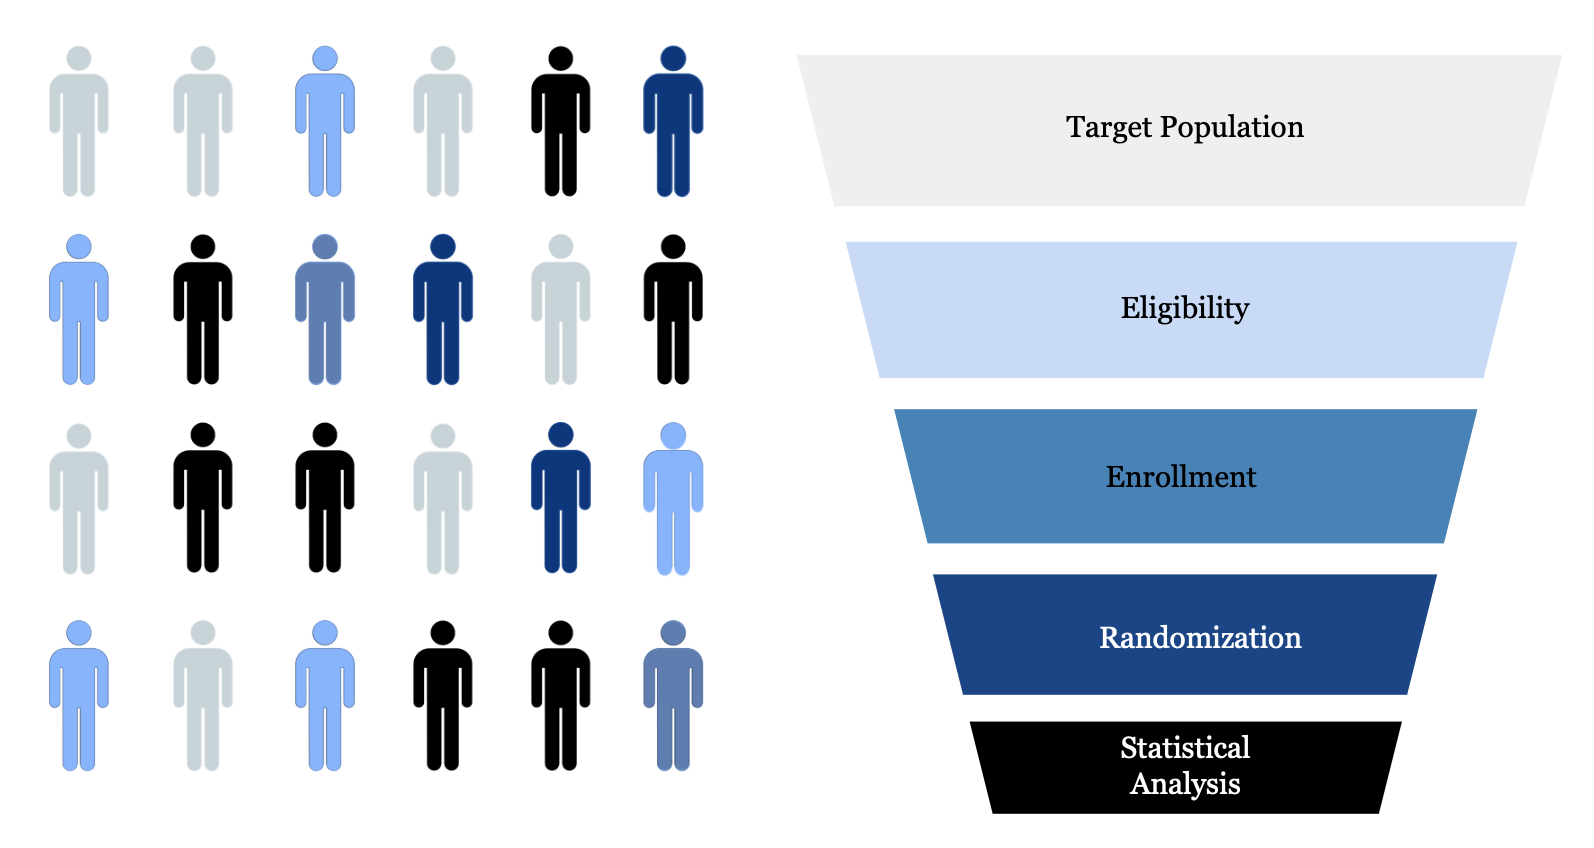
\includegraphics[width=100mm,scale=1]{statanal.png}

\end{frame}



\begin{frame}{Patient Leakage}

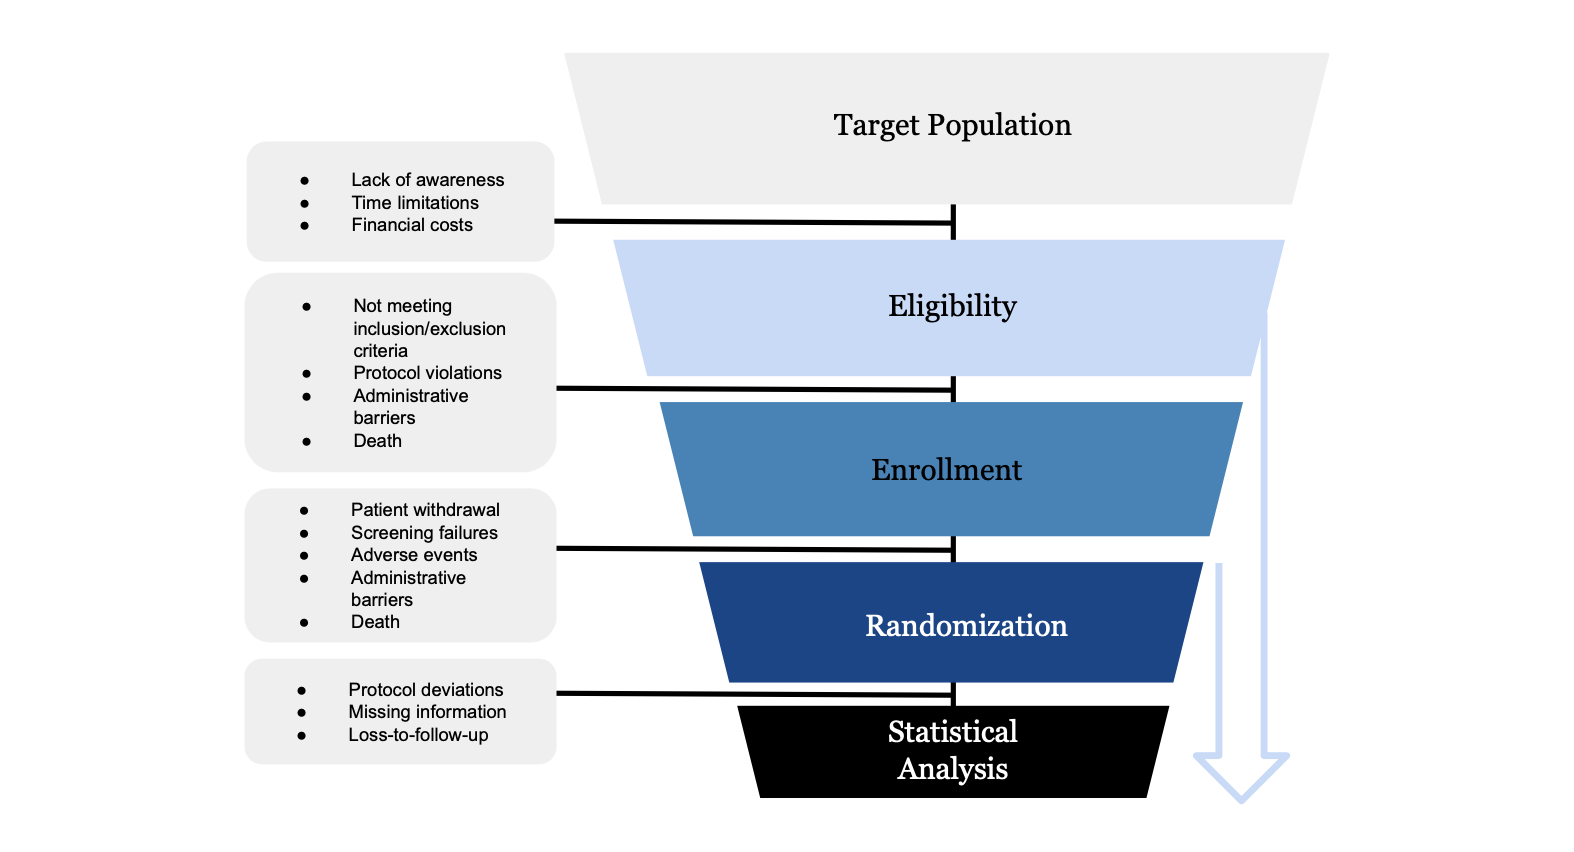
\includegraphics[width=100mm,scale=1]{attrition.png}

\end{frame}


\begin{frame}{Definitions}

\begin{itemize}
\item \textbf{Recruitment rate}: Per time-unit \citep{piantadosi2024clinical}
\begin{align*}
\lambda = \frac{\Delta C}{\Delta T} = \frac{C_1 - C_0}{T_1 - T_0} = \frac{C_1}{T_1}
\end{align*}

\item \textbf{Accrual}: Cumulative Recruitment
\item \textbf{Aleatory uncertainty}: randomness inherent and unpredictable
\item \textbf{Epistemic uncertainty}: arises from limited knowledge about recruitment rates



\end{itemize}


\end{frame}

\begin{frame}{Methods for Recruited Counts}

\end{frame}

\begin{frame}{Motivation Models for Counts}
\begin{figure}
\begin{knitrout}
\definecolor{shadecolor}{rgb}{0.969, 0.969, 0.969}\color{fgcolor}
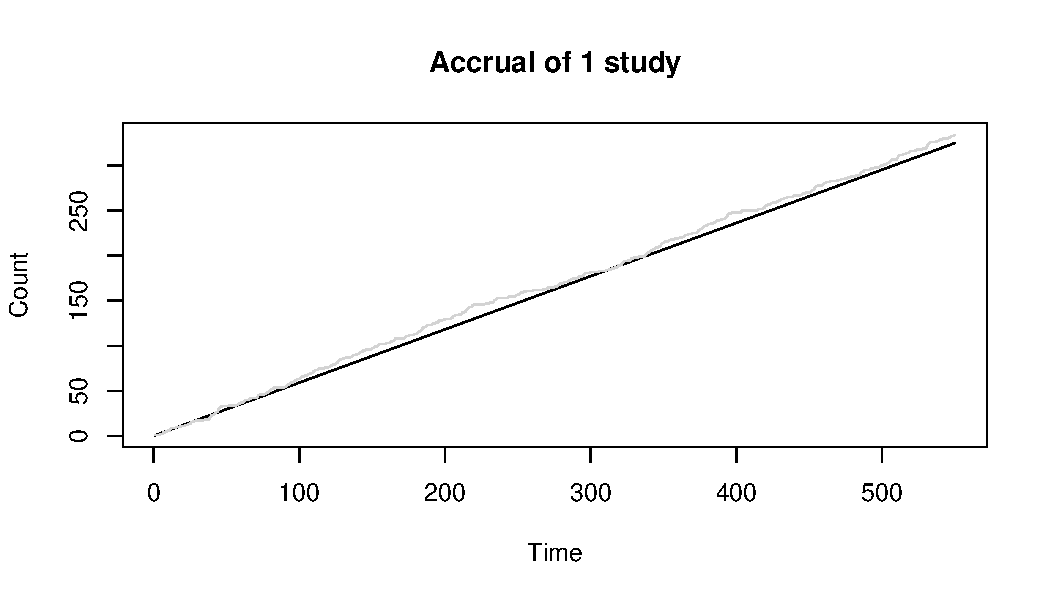
\includegraphics[width=\maxwidth]{figures/figunnamed-chunk-2-1} 
\end{knitrout}

\end{figure}

\end{frame}


\begin{frame}[shrink = 5]{Models for Counts}
\textbf{Recruitment} in unit of time (t=1):
\begin{table}[h!]
\centering
\resizebox{\textwidth}{!}{
\begin{tabular}{cccccc}
 \textbf{Methods} & \textbf{Counts} & \textbf{Expectation} & \textbf{Variance} & \textbf{Aleatory} & \textbf{Epistemic} \\
\hline
\hline
Expectation & $C = \lambda$ & $\lambda $ & 0 & No & No \\
Poisson & $C \sim$ Po $(\lambda )$ & $\lambda $ & $\lambda $ & Yes & No \\
Poisson - Gamma & $C \sim Po (\Lambda )$; $\Lambda \sim G(\alpha,\beta)$ & $\frac{\alpha}{\beta}$ & $\frac{\alpha(\beta+1)}{\beta^2}$ & Yes & Yes \\
\end{tabular}
}
\end{table}

\textbf{Accrual} for time t [0,t]:
\begin{table}[h!]
\centering
\resizebox{\textwidth}{!}{
\begin{tabular}{cccccc}
 \textbf{Methods} & \textbf{Counts} & \textbf{Expectation} & \textbf{Variance} & \textbf{Aleatory} & \textbf{Epistemic} \\
\hline
\hline
Expectation & $C(t) = \lambda  t$ & $\lambda  t$ & 0 & No & No \\
Poisson & $C(t) \sim Po (\lambda  t)$ & $\lambda  t$ & $\lambda  t$ & Yes & No \\
Poisson - Gamma & $C(t) \sim Po (\Lambda  t)$; $\Lambda \sim G(\alpha,\beta)$ & $t\frac{\alpha}{\beta}$ & $t\frac{\alpha(\beta+t)}{\beta^2}$ & Yes & Yes \\
\end{tabular}
}
\end{table}

\end{frame}

\begin{frame}{Multicenter Trial on Palliation in Terminal Esophageal Cancer}

Example from \cite{carter2004application}:
\begin{itemize}
\item Recruitment Rate $\lambda = 0.591$ per day
\item Time $Ttaget = 550$ days
\end{itemize}

\end{frame}


\begin{frame}{Multicenter Trial on Palliation in Terminal Esophageal Cancer}

Example from \cite{carter2004application}:
\begin{itemize}
\item Recruitment Rate $\lambda = 0.591$ per day
\item Time $Ttarget = 550$ days
\item Models for Counts at time point $t$:
	\begin{itemize}
	\item \textbf{Expectation}: $EC(t) = \lambda t$
	\item \textbf{Poisson}: $C(t) \sim Po(\lambda t)$
	\item \textbf{Poisson - Gamma}: $C(t) \sim Po (\Lambda t)$; $\Lambda \sim G(\alpha,\beta)$
	\begin{itemize}
	\item $\alpha = 32.4$ and $\beta = 54.8$
	\item $E\Lambda = \frac{\alpha}{\beta} = 0.591$
	\end{itemize}
	\end{itemize}
\end{itemize}

\end{frame}




\begin{frame}{Accrual at time point $t$}
\begin{itemize}
\item \textbf{Expectation}: $EC(t) = E\underbrace{(C +\ldots + C)}_{t \ \text{times}} = t E C = \lambda t$
\item \textbf{Poisson}: $\underbrace{Po (\lambda) +\ldots +Po (\lambda)}_{t \ \text{times}} = Po (\lambda t)$
% mention this is infinitely divisible property of poisson
\end{itemize}
\end{frame}


\begin{frame}{Accrual of 1 study}

\begin{figure}

\begin{knitrout}
\definecolor{shadecolor}{rgb}{0.969, 0.969, 0.969}\color{fgcolor}
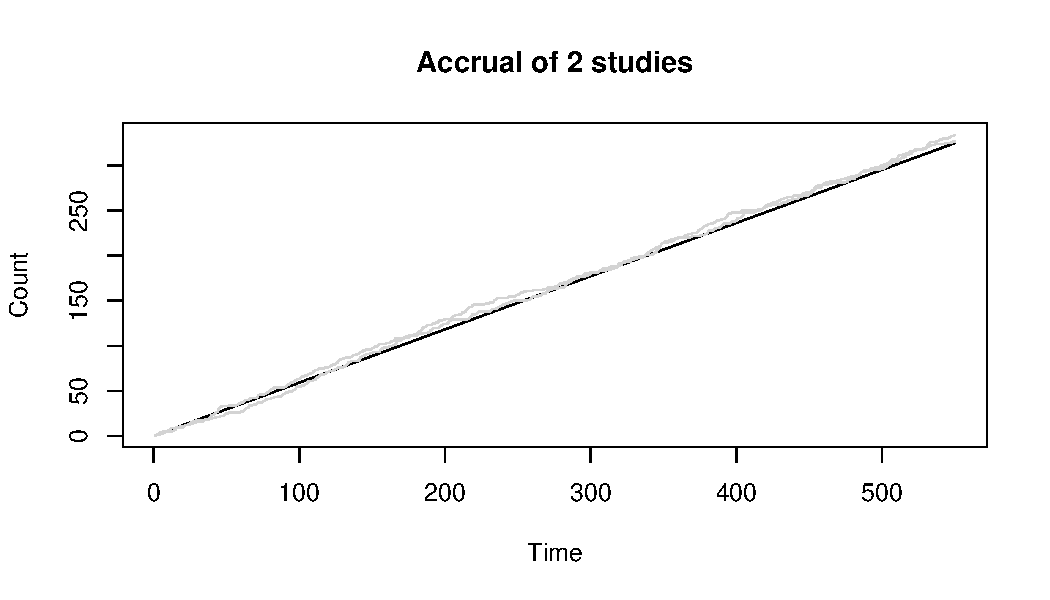
\includegraphics[width=\maxwidth]{figures/figunnamed-chunk-3-1} 
\end{knitrout}
 
\end{figure}


\end{frame}

\begin{frame}{Accrual of 2 studies}

\begin{figure}

\begin{knitrout}
\definecolor{shadecolor}{rgb}{0.969, 0.969, 0.969}\color{fgcolor}
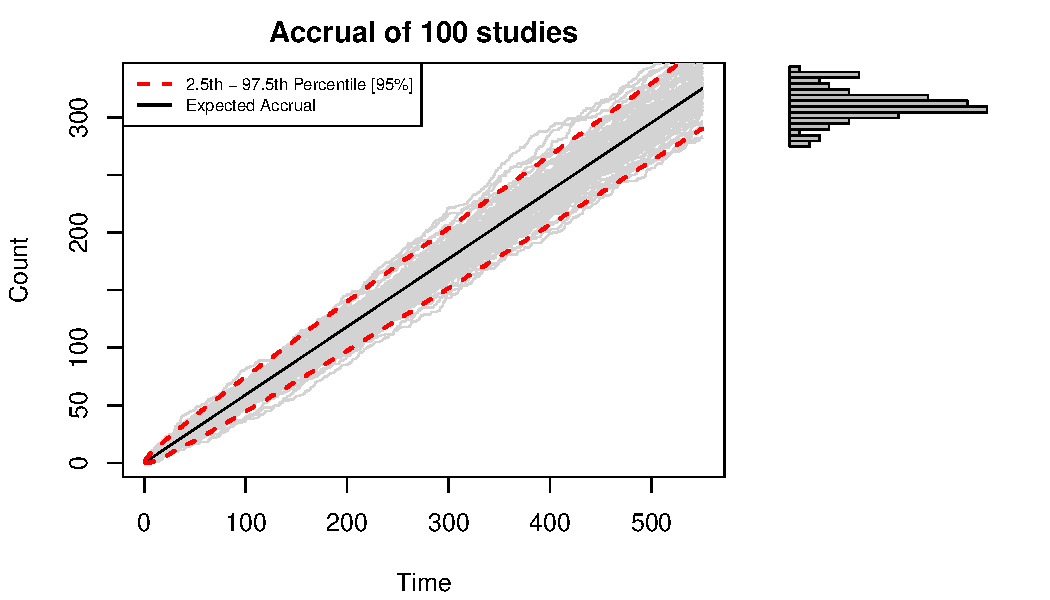
\includegraphics[width=\maxwidth]{figures/figunnamed-chunk-4-1} 
\end{knitrout}
  
\end{figure}


\end{frame}

% \begin{frame}{Accrual of 100 studies}
% 
% \begin{figure}
% <<echo=FALSE>>=
% # 1000 PATHS
% # Set parameters
% set.seed(2025)
% 
% n <- 100
% t <- seq(1, 550, 1)
% lambda <- 0.591
% 
% # Generate cumulative Poisson paths
% cval_cum_matrix <- matrix(NA, nrow = n, ncol = length(t))
% 
% for (i in 1:n) {
% 	cval <- rpois(length(t), lambda)  
% 	cval_cum_matrix[i, ] <- cumsum(cval)  
% }
% 
% # Extract final counts for histogram
% final_counts <- cval_cum_matrix[, length(t)]
% 
% 
% # Reset graphics device to avoid layout issues
% # if (dev.cur() > 1) dev.off()
% 
% # Set up layout: Histogram (small, upper right) + Main plot
% layout(matrix(c(1, 2), ncol = 2), widths = c(3, 1), heights = c(4, 1))  
% 
% # Plot the main accrual time series
% par(mar = c(4.1, 4.1, 2.1, 2.1))  # Restore normal margins
% plot(t,  cval_cum_matrix[1,], 
% 		 type="n", 
% 		 main = "Accrual of 100 studies", 
% 		 xlab = "Time", 
% 		 ylab = "Count")
% 
% for(i in 1:n){
% 	lines(t,  cval_cum_matrix[i,], col = "lightgray")
% }
% 
% # Add reference lines
% lines(t, lambda*t)
% lines(t, qpois(p = 0.975, lambda*t), lty = 2, lwd = 2, col = "red")
% lines(t, qpois(p = 0.025, lambda*t), lty = 2, lwd = 2, col = "red")
% 
% 
% legend("topleft",
% 			 legend = c("2.5th - 97.5th Percentile [95%]",
% 			 					 "Expected Accrual"),
% 			 col = c("red", "black"),
% 			 lty = c(2, 1),
% 			 lwd = c(2,2),
% 			 bg = "white",
% 			 cex = 0.7)  
% 
% # Plot histogram in the smaller upper right section
% par(mar = c(15, 0.01, 2.1, 2.1))  # Minimize margins
% hist_bins <- seq(min(final_counts), max(final_counts), length.out = 15)
% hist_data <- hist(final_counts, breaks = hist_bins, plot = FALSE)
% 
% 
% barplot(hist_data$counts, horiz = TRUE, space = 0, col = "gray", 
% 				axes = FALSE, xlab = "", ylab = "")
% @   
% 
% \end{figure}
% 
% \end{frame}

\begin{frame}{Accrual of 100 studies}

\begin{figure}
\begin{knitrout}
\definecolor{shadecolor}{rgb}{0.969, 0.969, 0.969}\color{fgcolor}
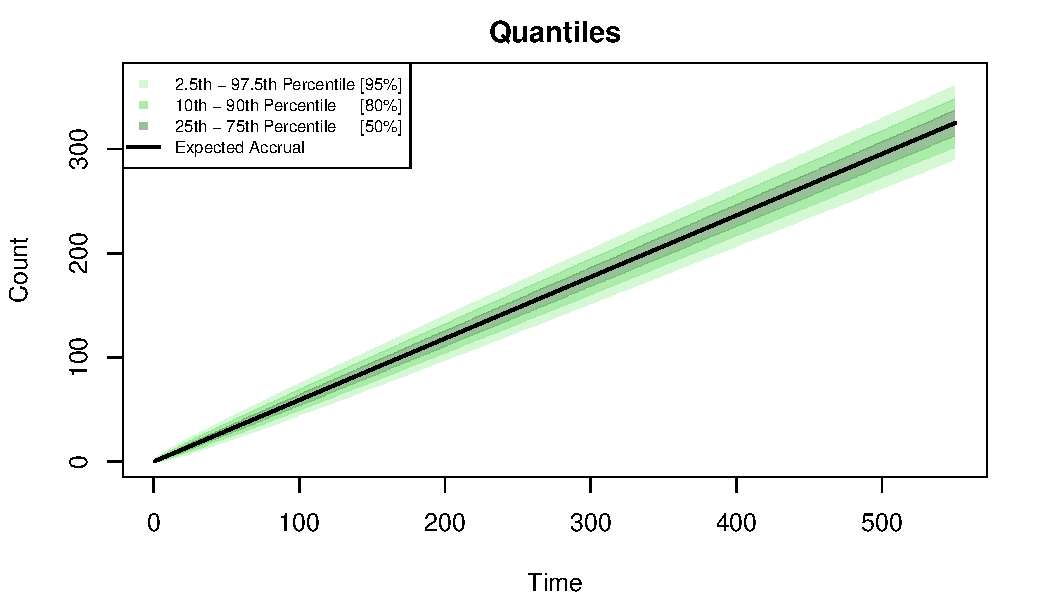
\includegraphics[width=\maxwidth]{figures/figunnamed-chunk-5-1} 
\end{knitrout}

\end{figure}

\end{frame}

\begin{frame}{Exact Poisson's and Poisson-Gamma's uncertainty bands}
\begin{figure}
\begin{knitrout}
\definecolor{shadecolor}{rgb}{0.969, 0.969, 0.969}\color{fgcolor}
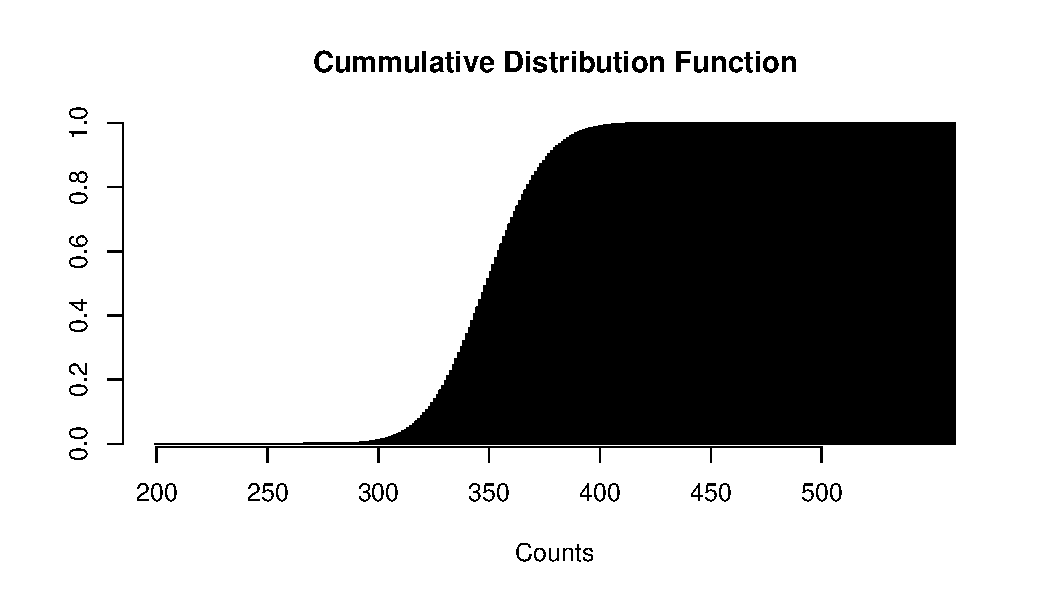
\includegraphics[width=\maxwidth]{figures/figunnamed-chunk-6-1} 
\end{knitrout}
\end{figure}
\end{frame}


% \begin{frame}{Poisson's uncertainty bands}
% 
% 
% \begin{figure}
% <<echo=FALSE>>=
% 
% # Compute Poisson quantiles over time
% q_975_line <- qpois(0.975, lambda * t)
% q_900_line <- qpois(0.900, lambda * t)
% q_750_line <- qpois(0.75, lambda * t)
% q_250_line <- qpois(0.25, lambda * t)
% q_100_line <- qpois(0.1, lambda * t)
% q_025_line <- qpois(0.025, lambda * t)
% 
% # Define x and y axis limits
% x_limits <- range(t)
% y_limits <- range(cval_cum_matrix)  # Ensures all quantiles fit
% 
% # Create the plot
% par(mar = c(4.1, 4.1, 2.1, 2.1))
% plot(NA, NA, xlim = x_limits, ylim = y_limits, xlab = "Time", ylab = "Count",
% 		 main = "Quantiles")
% 
% # Fill the area with a green gradient
% polygon(c(t, rev(t)), c(q_975_line, rev(q_900_line)), col = rgb(144/255, 238/255, 144/255, 0.4), border = NA) # Light Green
% polygon(c(t, rev(t)), c(q_900_line, rev(q_750_line)), col = rgb(50/255, 205/255, 50/255, 0.4), border = NA)  # Lime Green
% polygon(c(t, rev(t)), c(q_750_line, rev(q_250_line)), col = rgb(0/255, 100/255, 0/255, 0.4), border = NA)    # Dark Green
% polygon(c(t, rev(t)), c(q_250_line, rev(q_100_line)), col = rgb(50/255, 205/255, 50/255, 0.4), border = NA)  # Lime Green
% polygon(c(t, rev(t)), c(q_100_line, rev(q_025_line)), col = rgb(144/255, 238/255, 144/255, 0.4), border = NA) # Light Green
% 
% # Add the mean trend line
% lines(t, lambda * t, col = "black", lwd = 2)  
% 
% # Legend
% legend("topleft",
% 			 legend = c("2.5th - 97.5th Percentile [95%]", 
% 			 					 "10th - 90th Percentile     [80%]", 
% 			 					 "25th - 75th Percentile     [50%]", 
% 			 					 "Expected Accrual"),
% 			 col = c(rgb(144/255, 238/255, 144/255, 0.4), rgb(50/255, 205/255, 50/255, 0.4), rgb(0/255, 100/255, 0/255, 0.4), "black"),
% 			 pch = c(15, 15, 15, NA), lty = c(NA, NA, NA, 1), lwd = c(NA, NA, NA, 2),
% 			 bg = "white",
% 			 cex = 0.7)
% @   
% \end{figure}
% 
% \end{frame}
% 


% \begin{frame}{Poisson's exact PMF at time point $t=550$ with $\lambda = 0.591$}
% \begin{figure}
% <<echo=FALSE>>=
% bar_positions <- barplot(dpois(200:500, lambda*550), 
% 												 main = "Probability Mass Function", 
% 												 xlab = "Counts", 
% 												 xaxt = "n")  
% 
% axis(1, at = seq(1, length(200:500), by = 50), labels = seq(200, 500, by = 50))  
% @   
%   \caption{Poisson Distribution of Counts: This bar plot represents the probability mass function (PMF) of counts ranging from 200 to 500, using a Poisson distribution with a rate parameter $\lambda = 0.591$ based on 550 time periods.}
%   \label{fig:2_3}
% \end{figure}
% \end{frame}

% \begin{frame}{Poisson's exact CDF at time point $t=550$ with $\lambda = 0.591$}
% 
% \begin{figure}
% <<echo=FALSE>>=
% probdist <- dpois(200:500, lambda*550)
% cdf <- cumsum(probdist)
% cdf_positions <- barplot(cdf, 
% 												 main = "Cummulative Distribution Function", 
% 												 xlab = "Counts", 
% 												 xaxt = "n")
% axis(1, at = seq(1, length(200:500), by = 50), labels = seq(200, 500, by = 50))  
% @   
%   \caption{Cumulative Distribution of Poisson-Distributed Counts: The plot illustrates the cumulative probability distribution for counts within the range of 200 to 500, using a Poisson distribution with a rate parameter $\lambda = 0.591$ adjusted for 550 time periods.}
%   \label{fig:2_4}
% \end{figure}
% \end{frame}




% \begin{frame}{Multicenter Trial on Palliation in Terminal Esophageal Cancer}
% Example from \cite{carter2004application}:
% \begin{itemize}
% \item Recruitment Rate $\lambda = \frac{Counts}{Time} = 0.591$ per day
% \item Time $t = 550$ days
% \item Models for Counts at time point $t$:
% 	\begin{itemize}
% 	\item \textbf{Poisson - Gamma}: $C(t) \sim Po (\Lambda t)$; $\Lambda \sim G(\alpha,\beta)$
% 		\begin{itemize}
% 		\item $\alpha = 325$
% 		\item $\beta = 548$
% 		\item $E \Lambda = \frac{\alpha}{\beta} = 0.591 = \lambda$
% 		\end{itemize}
% 	\end{itemize}
% \end{itemize}
% \end{frame}

\begin{frame}{Two versions of randomness of $\Lambda$}
\begin{itemize}
\item \textbf{Version 1:} Random recruitment rate realization $\lambda$ varies across studies and remains \textbf{fixed} within study \textbf{over time} \\ $\rightarrow$ PoG distribution
\item \textbf{Version 2:} Random recruitment rate realization $\lambda$ varies across studies and \textbf{varies} within study \textbf{over time} \\ $\rightarrow$ Distribution with unexpected properties
\end{itemize}
\end{frame}

\begin{frame}{Version 1 different from Version 2}
\begin{figure}
\begin{knitrout}
\definecolor{shadecolor}{rgb}{0.969, 0.969, 0.969}\color{fgcolor}
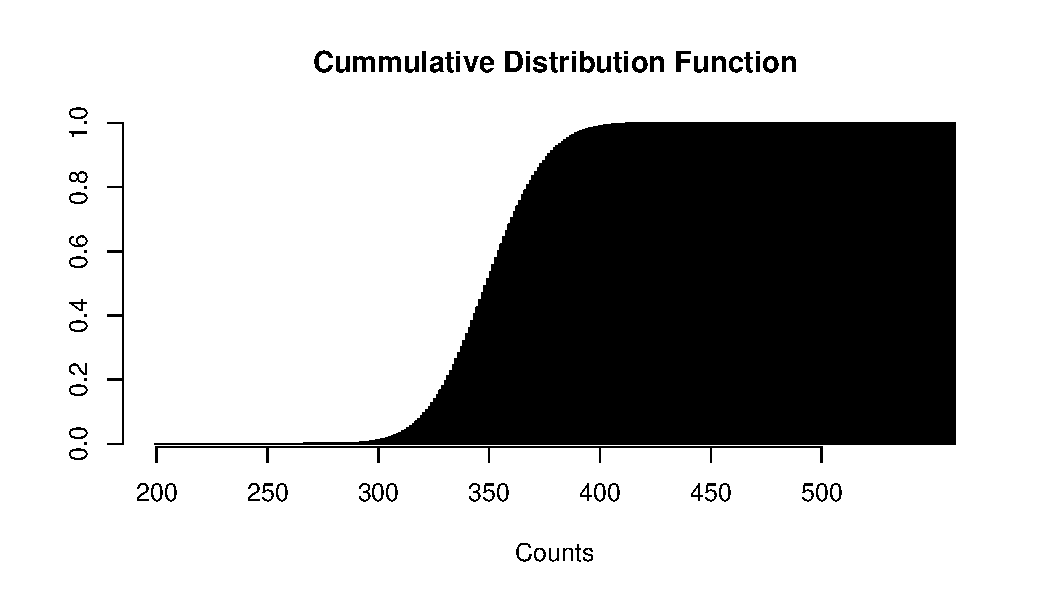
\includegraphics[width=\maxwidth]{figures/figunnamed-chunk-7-1} 
\end{knitrout}

\end{figure}
\end{frame}

\begin{frame}[shrink = 5]{Negative binomial derived from Poisson-Gamma model at time point $t$}

Let $C(t)|\Lambda \sim Po(\Lambda t)$ and $\Lambda \sim G(\alpha,\beta)$
\begin{align*}
p(c)&=\int^\infty_0 p(c|\lambda) p(\lambda) d\lambda\\
&=\int^\infty_0 \frac{(\lambda t)^c\exp(-\lambda t)}{c!}\Bigg[(\lambda)^{\alpha-1}\exp(-\beta\lambda)\frac{\beta^\alpha}{\Gamma(\alpha)}\Bigg]d\lambda\\
&=\frac{\beta^\alpha t^c \Gamma(\alpha+c)}{c!\Gamma(\alpha) (\beta+t)^{\alpha+c}}\underbrace{\int^\infty_0 \frac{(\beta+t)^{\alpha+c}}{\Gamma(\alpha+c)} \lambda^{\alpha+c-1}\exp(-(\beta+t)\lambda)d\lambda}_{=1}\\
&=\binom{\alpha+c-1}{\alpha-1}\Bigg (\frac{t}{\beta+t}\Bigg)^{c} \Bigg(\frac{\beta}{\beta+t}\Bigg)^{\alpha}, \\
C(t)\sim NBin \Bigg(\alpha, \frac{\beta}{\beta+t}\Bigg)
\end{align*}
% talk here about interpretations (from report)
\end{frame}


\begin{frame}{Expectation and Variance for Counts}
Using the expressions of iterated expectation and variance \citep{held2014applied}

\begin{align*}
E(C(t)) &= E_{\Lambda}[E_{C(t)} (C(t)|\Lambda)] = E_{\Lambda}[\Lambda t] = t\alpha/\beta
\end{align*}

\begin{align*}
Var(C(t)) &= Var_{\Lambda}[E_{C(t)} (C(t)|\Lambda)] + E_{\Lambda}[Var_{C(t)}(C(t)|\Lambda)]\\
&=Var_{\Lambda}[\Lambda t] + E_{\Lambda}[\Lambda t] \\
&=t^2\alpha/\beta^2 + t\alpha/\beta = \frac{t \alpha(\beta+t)}{\beta^2}
\end{align*}
\end{frame}

% \begin{frame}{Gamma Prior}
% $\Lambda \sim G(\alpha,\beta)$
% <<echo = FALSE>>=
% curve(dgamma(x, shape = 324, rate = 548), 
% 			from = 0, to = 1,
% 			main = "Probability Density Function", 
% 			xlab = "Recruitment rate", 
% 			ylab = "",
% 			col = "red")
% 
% 
% legend("topleft",
% 			 legend = c(expression("G(" ~ alpha == 324 ~ beta == 548 ~ ")")),
% 			 col = c("red"),
% 			 lty = c(1, 1),
% 			 bg = "white",
% 			 cex = 0.6)
% @
% 
% \end{frame}
% 
% 
% \begin{frame}{Comparison between Poisson and Poisson - Gamma}
% \begin{figure}
% <<echo=FALSE>>=
% plot(200:500, dpois(200:500, lambda*550), 
% 		 type = "l",
% 		 main = "Probability Mass Function", 
% 		 xlab = "Counts", 
% 		 ylab = "")
% 
% alpha = 324
% beta = 1.5 * 365
% 
% lines(200:500, dnbinom(200:500, size = 324, mu = lambda*550), col = "red")
% 
% legend("topleft",
% 			 legend = c(expression(Po(lambda == 0.591)),
%                   expression(PoG ~ (alpha == 324 ~ beta == 548))),
% 			 col = c("black", "red"),
% 			 lty = c(1, 1),
% 			 bg = "white",
% 			 cex = 0.6) 
% @   
%   \caption{Comparison of Probability Mass Function (PMF) between Poisson distribution with $\lambda = 0.591$ and Negative Binomial with $\alpha = 324$ and $\mu = 0.591$.}
%   \label{fig:2_6}
% \end{figure}
% \end{frame}
% 
% 
% \begin{frame}{Comparison between Poisson and Poisson - Gamma}
% 
% \begin{figure}
% <<echo=FALSE>>=
% plot(200:500, ppois(200:500, lambda*550), 
% 		 type = "l",
% 		 main = "Cummulative Distribution Function", 
% 		 xlab = "Counts", 
% 		 ylab = "")
% 
% alpha = 324
% beta = 1.5 * 365
% 
% lines(200:500, pnbinom(200:500, size = 324, mu = lambda*550), col = "red")
% 
% legend("topleft",
% 			 legend = c(expression(Po(lambda == 0.591)),
%                   expression(PoG ~ (alpha == 324 ~ beta == 548))),
% 			 col = c("black", "red"),
% 			 lty = c(1, 1),
% 			 bg = "white",
% 			 cex = 0.6)
% @   
%   \caption{Comparison of Cummulative Distribution Function (CDF) between Poisson distribution with $\lambda = 0.591$ and Negative Binomial with $\alpha = 324$ and $\mu = 0.591$.}
%   \label{fig:2_7}
% \end{figure}
% 
% \end{frame}

\begin{frame}{Sensitivity Analysis}


\end{frame}


\begin{frame}{Sensitivity Analysis}
\begin{knitrout}
\definecolor{shadecolor}{rgb}{0.969, 0.969, 0.969}\color{fgcolor}
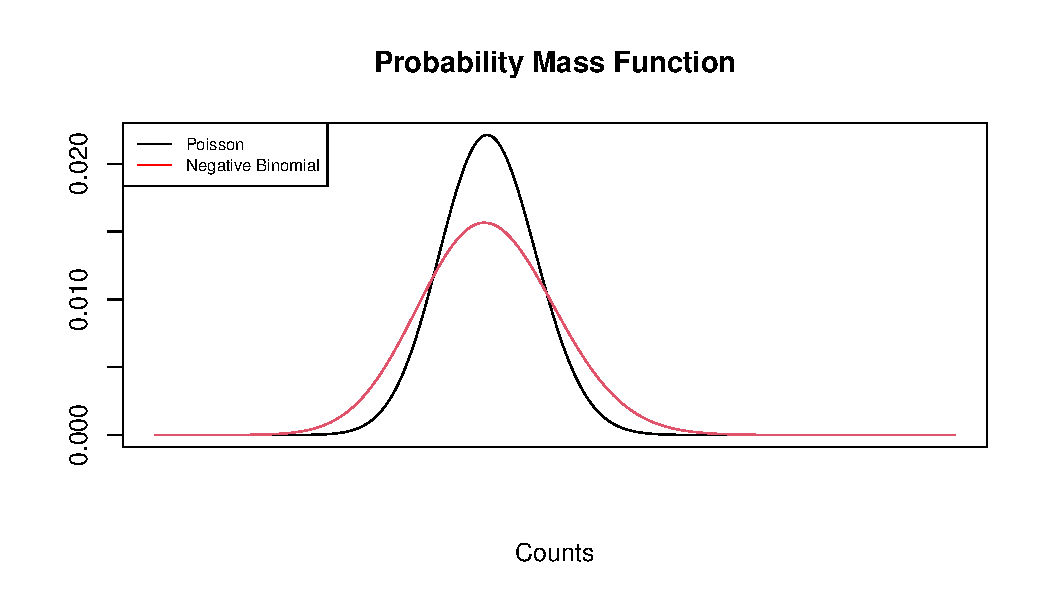
\includegraphics[width=\maxwidth]{figures/figunnamed-chunk-8-1} 
\end{knitrout}

\end{frame}


\begin{frame}{Sensitivity Analysis}
\begin{knitrout}
\definecolor{shadecolor}{rgb}{0.969, 0.969, 0.969}\color{fgcolor}
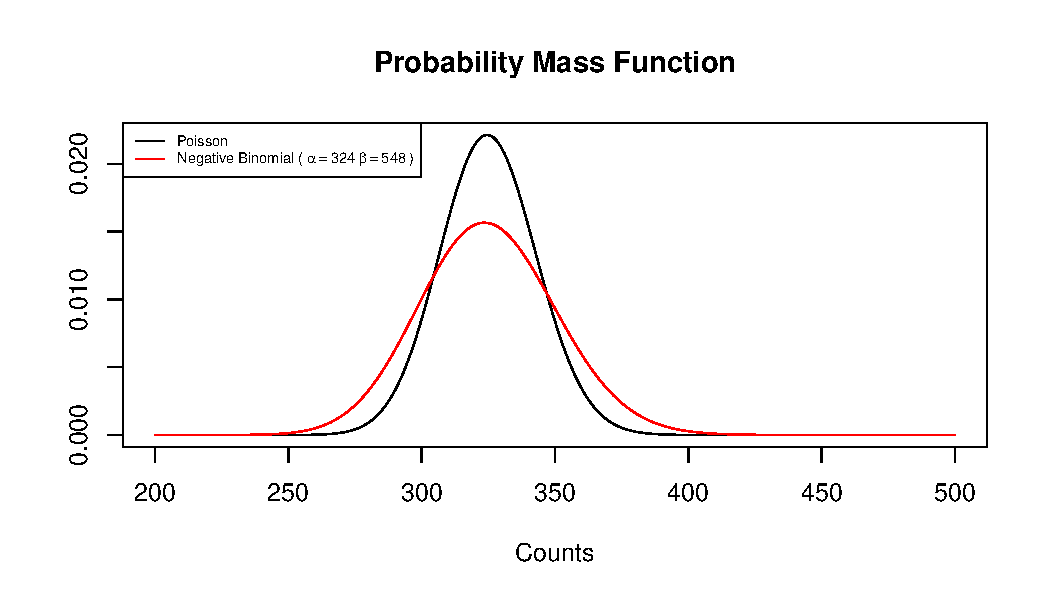
\includegraphics[width=\maxwidth]{figures/figunnamed-chunk-9-1} 
\end{knitrout}

\end{frame}



\begin{frame}{Sensitivity Analysis}
\begin{knitrout}
\definecolor{shadecolor}{rgb}{0.969, 0.969, 0.969}\color{fgcolor}
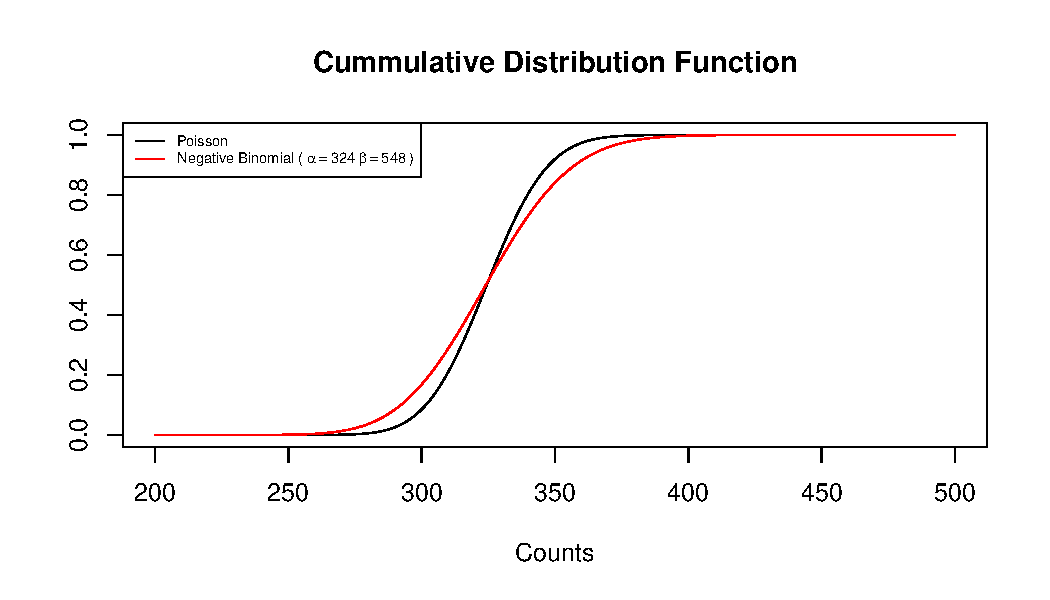
\includegraphics[width=\maxwidth]{figures/figunnamed-chunk-10-1} 
\end{knitrout}

\end{frame}


% 
% \begin{frame}[shrink = 5]{Models for Counts}
% \textbf{Recruitment} in unit of time (t=1):
% \begin{table}[h!]
% \centering
% \resizebox{\textwidth}{!}{
% \begin{tabular}{cccccc}
%  \textbf{Methods} & \textbf{Counts} & \textbf{Expectation} & \textbf{Variance} & \textbf{Aleatory} & \textbf{Epistemic} \\
% \hline
% \hline
% Expectation & $C = \lambda$ & $\lambda $ & 0 & No & No \\
% Poisson & $C \sim$ Po $(\lambda )$ & $\lambda $ & $\lambda $ & Yes & No \\
% Poisson - Gamma & $C \sim Po (\Lambda )$; $\Lambda \sim G(\alpha,\beta)$ & $\frac{\alpha}{\beta}$ & $\frac{\alpha(\beta+1)}{\beta^2}$ & Yes & Yes \\
% \end{tabular}
% }
% \end{table}

% \textbf{Accrual} for time t [0,t]:
% \begin{table}[h!]
% \centering
% \resizebox{\textwidth}{!}{
% \begin{tabular}{cccccc}
%  \textbf{Methods} & \textbf{Counts} & \textbf{Expectation} & \textbf{Variance} & \textbf{Aleatory} & \textbf{Epistemic} \\
% \hline
% \hline
% Expectation & $C(t) = \lambda  t$ & $\lambda  t$ & 0 & No & No \\
% Poisson & $C(t) \sim Po (\lambda  t)$ & $\lambda  t$ & $\lambda  t$ & Yes & No \\
% Poisson - Gamma & $C(t) \sim Po (\Lambda  t)$; $\Lambda \sim G(\alpha,\beta)$ & $t\frac{\alpha}{\beta}$ & $t\frac{\alpha(\beta+t)}{\beta^2}$ & Yes & Yes \\
% \end{tabular}
% }
% \end{table}
% 
% \end{frame}

\begin{frame}{Methods for Waiting Time}

\end{frame}

\begin{frame}{Motivation Models for Waiting Time}
\begin{figure}
\centering
\begin{knitrout}
\definecolor{shadecolor}{rgb}{0.969, 0.969, 0.969}\color{fgcolor}
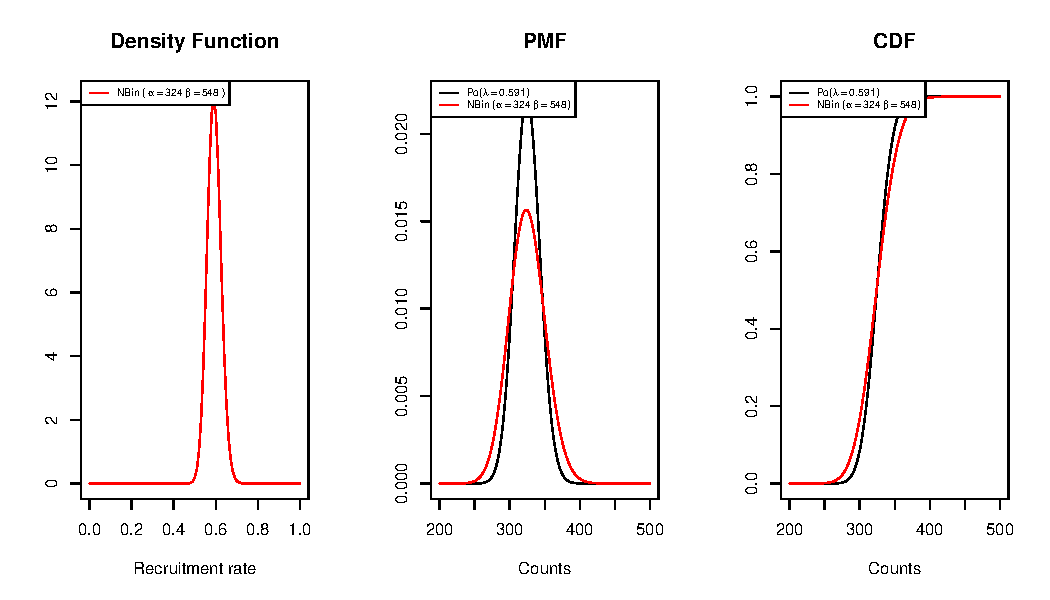
\includegraphics[width=\maxwidth]{figures/figunnamed-chunk-11-1} 
\end{knitrout}

\end{figure}
\end{frame}

\begin{frame}{Models for Waiting Time until Target Sample Size $c$}
\begin{table}[h!]
\centering
\resizebox{\textwidth}{!}{
\begin{tabular}{cccccc}
 \textbf{Methods} & \textbf{Time} & \textbf{Expectation} & \textbf{Variance} & \textbf{Aleatory} & \textbf{Epistemic} \\
\hline
\hline
Expectation & $T(c) = c/\lambda$ & $c/\lambda$ & 0 & No & No \\
Erlang & $T(c) \sim \textrm{G}(c, \lambda) $ & $c/\lambda$ & $c/\lambda^2$ & Yes & No \\
Gamma-Gamma & $T(c) \sim \textrm{G}(c, \Lambda)$; $\Lambda \sim \textrm{G}(\alpha,\beta)$ & $c\frac{\beta}{\alpha-1}$ & $\frac{c\beta^2(c+\alpha-1)}{(\alpha-1)^2(\alpha-2)}$ & Yes & Yes \\
\end{tabular}
}
\end{table}

\begin{itemize}
\item Two versions of randomness of $\Lambda$
\item Version 1 $\rightarrow$ GG distribution 
\item Similar derivations as shown for counts
\end{itemize}
\end{frame}

% \begin{frame}
% \begin{align*}
% p(t) &= \int_0^{\infty} p(t|\lambda) p(\lambda) d\lambda\\
% &= \int_0^{\infty}\Bigg( \frac{\lambda^ct^{c-1}\exp(-\lambda t)}{\Gamma(c)}\Bigg)\Bigg(\frac{\beta^{\alpha}\lambda^{\alpha-1}\exp(-\beta \lambda)}{\Gamma(\alpha)}\Bigg)d\lambda \\
% &=\frac{t^{c-1}\beta^{\alpha}}{\Gamma(c)\Gamma(\alpha)}\int_0^{\infty}\lambda^{c+\alpha-1}\exp(-\lambda(\beta+t))d\lambda\\
% &=\frac{\Gamma(\alpha+c)}{\Gamma(c)\Gamma(\alpha)}\frac{t^{c-1}\beta^{\alpha}}{(\beta+t)^{\alpha+c}}\underbrace{\int_0^{\infty}\frac{(\beta+t)^{\alpha+c}}{\Gamma(\alpha+c)}\lambda^{c+\alpha-1}\exp(-\lambda(\beta+t))d\lambda}_{=1}\\
% &=\frac{\Gamma(\alpha+c)}{\Gamma(c)\Gamma(\alpha)}\frac{t^{c-1}\beta^{\alpha}}{(\beta+t)^{\alpha+c}}\\
% &=\frac{\beta^{\alpha}}{\B(\alpha, c)}\frac{t^{c-1}}{(\beta+t)^{\alpha+c}}
% \end{align*}
% \end{frame}


% \begin{frame}[shrink=5]{Expectation and Variance for Waiting Times}
% Using the expressions of iterated expectation and variance \citep{held2014applied} and that when $\Lambda \sim \textrm{G}(\alpha, \beta)$ then, $\frac{1}{\Lambda} \sim \textrm{IG}(\alpha, \beta)$
% 
% \begin{align*}
% \textrm{E}T(c) &= \textrm{E}_{\Lambda}[\textrm{E}_{T(c)} (T(c)|\Lambda)] = \textrm{E}_{\Lambda}\Bigg [\frac{c}{\Lambda}\Bigg ] = c \textrm{E}_{\Lambda}\Bigg [\frac{1}{\Lambda}\Bigg ] = c\frac{\beta}{\alpha-1}, \ \alpha>1
% \end{align*}
% 
% 
% \begin{align*}
% \textrm{Var}(T(c)) &= \textrm{Var}_{\Lambda}[\textrm{E}_{T(c)} (T(c)|\Lambda)] + \textrm{E}_{\Lambda}[\textrm{Var}_{T(c)}(T(c)|\Lambda)]\\
% &=\textrm{Var}_{\Lambda}\Bigg [\frac{c}{\Lambda}\Bigg ] + \textrm{E}_{\Lambda}\Bigg [\frac{c}{\Lambda^2}\Bigg ] \\
% &=c^2\textrm{Var}_{\Lambda}\Bigg [\frac{1}{\Lambda}\Bigg ] + c\textrm{E}_{\Lambda}\Bigg [\frac{1}{\Lambda^2}\Bigg ] \\
% %&=\frac{c^2\beta^2}{(\alpha-1)^2(\alpha-2)} + \frac{c\beta^2}{(\alpha-1)(\alpha-2)}\\
% &=\frac{c\beta^2(c+\alpha-1)}{(\alpha-1)^2(\alpha-2)}, \ \alpha>2
% \end{align*}
% \end{frame}

\begin{frame}{Sensitivity Analysis for Waiting Time}

\begin{figure}
\centering
\begin{knitrout}
\definecolor{shadecolor}{rgb}{0.969, 0.969, 0.969}\color{fgcolor}
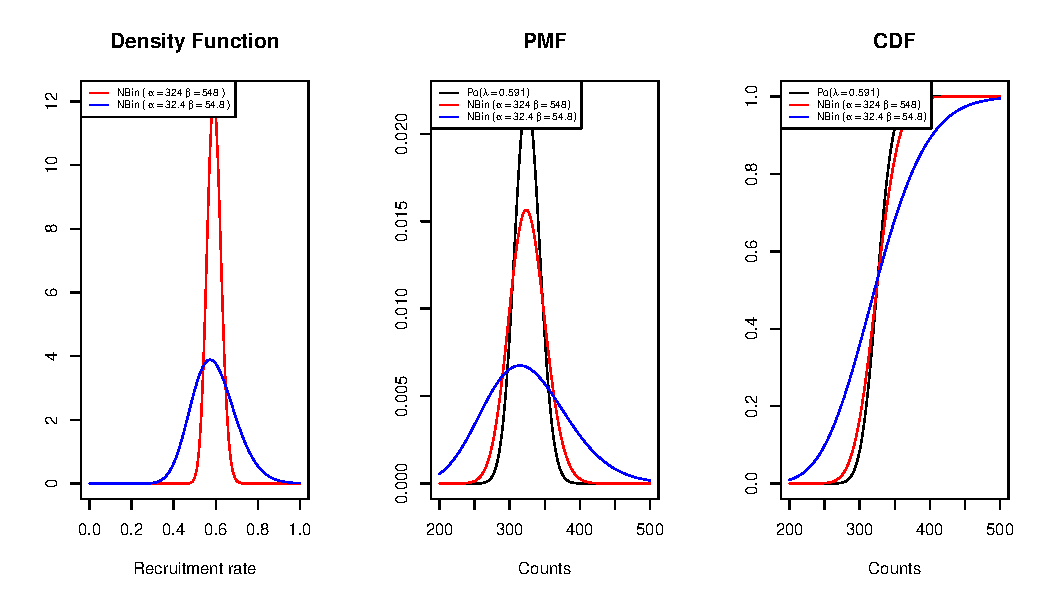
\includegraphics[width=\maxwidth]{figures/figunnamed-chunk-12-1} 
\end{knitrout}
\end{figure}
\end{frame}

\begin{frame}{Exact Methods vs MC simulations}

\end{frame}

% 
% \begin{frame}[shrink=20]{Exact Methods vs MC simulations}
% <<echo=FALSE, cache = TRUE, warning=FALSE>>=
% set.seed(2025)
% 
% M <- 10^4
% t <- seq(1, 550, 1)
% lambda <- 0.591
% 
% # Generate cumulative Poisson paths
% cval_cum_matrix <- matrix(NA, nrow = M, ncol = length(t))
% 
% for (i in 1:M) {
% 	cval <- rpois(length(t), lambda)  
% 	cval_cum_matrix[i, ] <- cumsum(cval)  
% }
% 
% # Extract final counts for histogram
% final_counts_p <- cval_cum_matrix[, length(t)]
% 
% set.seed(2025)
% 
% n <- 10^4
% t <- seq(1, 550, 1)
% lambda <- 0.591
% 
% alpha <- 32.4
% beta <- 54.8
% # Generate cumulative Poisson paths
% cval_cum_matrix <- matrix(NA, nrow = n, ncol = length(t))
% v_lambda <- rgamma(n, shape = alpha, rate = beta)
% 
% for (i in 1:n) {
% 	cval <- rpois(length(t), lambda = v_lambda[i])
% 	cval_cum_matrix[i, ] <- cumsum(cval)  
% }
% 
% # Extract final counts for histogram
% final_counts_pg <- cval_cum_matrix[, length(t)]
% 
% M <- 10^4
% Ctarget <- 324
% lambda <- 0.591
% 
% alpha <- 32.4
% beta <- 54.8
% 
% simulate_time_to_threshold_Erlang_easier <- function(MM, CC, ll, rseed=265735) {
%   set.seed(rseed)
%   timeerlang <- rgamma(n=MM, shape = CC, rate = ll)
%   return(timeerlang)
% }
% 
% time_erlang <- simulate_time_to_threshold_Erlang_easier(MM=M, CC=Ctarget, ll=lambda, rseed=265735)
% 
% set.seed(2025)
% M <- 10^4
% Ctarget <-324 
% lambda <- 0.591
% alpha <- 32.4
% beta <- 54.8
% 
% simulate_time_to_threshold_GG_easier <- function(MM, CC, aa, bb, rseed=265735) {
%   set.seed(rseed)
%   timegg <- rep(0, MM)
%   lambdar <- rgamma(n=MM, shape = aa, rate = bb)
%   for (i in 1:MM){
%     timegg[i] <- rgamma(n=1, shape = CC, rate = lambdar[i])
%   }
%   return(timegg)
% }
% 
% timegg_easier <- simulate_time_to_threshold_GG_easier(MM=M, CC=Ctarget, aa=alpha, bb=beta) 
% 
% @
% \begin{table}[h!]
% \centering
% \begin{tabular}{cccc}
%  \textbf{Model} & \textbf{Estimated Probabilty} & \textbf{MCse} & \textbf{Exact Probability} \\
% \hline
% \hline
%  $C(T)\sim\textrm{Po}(\lambda T)$ & $\textrm{P}(C(T)\geq 324) = round(mean(final_counts_p>324),3)$ & round(sqrt(mean(final_counts_p>324)*(1-mean(final_counts_p>324))/M), 3) & round(1-ppois(324, lambda*550),3) \\
%  $C(T)\sim\textrm{PoG}(T, \alpha, \beta)$ & $\textrm{P}(C(T)\geq 324) = round(mean(final_counts_pg>324),3)$ & round(sqrt(mean(final_counts_pg>324)*(1-mean(final_counts_pg>324))/M), 3) & round(1-pnbinom(324, size = 324, mu = lambda * 550),3) 
% \end{tabular}
% \end{table}
% 
% \begin{table}[h!]
% \centering
% \begin{tabular}{cccc}
%  \textbf{Model} & \textbf{Estimated Probabilty} & \textbf{MCse} & \textbf{Exact Probability} \\
% \hline
% \hline
%  $T(C)\sim\textrm{G}(C, \lambda)$& $\textrm{P}(T(C)\geq 548) = round(mean(time_erlang>548),3)$ & round(sqrt(mean(time_erlang>548)*(1-mean(time_erlang>548))/M), 3) & round(1-pgamma(548, shape = 324, rate = lambda),3)\\
% $T(C)\sim\textrm{GG}(C, \alpha, \beta)$ & $\textrm{P}(T(C)\geq 548) = round(mean(timegg_easier>548),3)$ & round(sqrt(mean(timegg_easier>548)*(1-mean(timegg_easier>548))/M), 3) & round(1-pgammagamma(548, alpha = alpha, b = beta, c = 324),3)
% \end{tabular}
% \end{table}
% 
% \end{frame}




\begin{frame}{Exact Methods vs MC simulations -- Poisson-Gamma Counts}

\begin{figure}
\begin{knitrout}
\definecolor{shadecolor}{rgb}{0.969, 0.969, 0.969}\color{fgcolor}
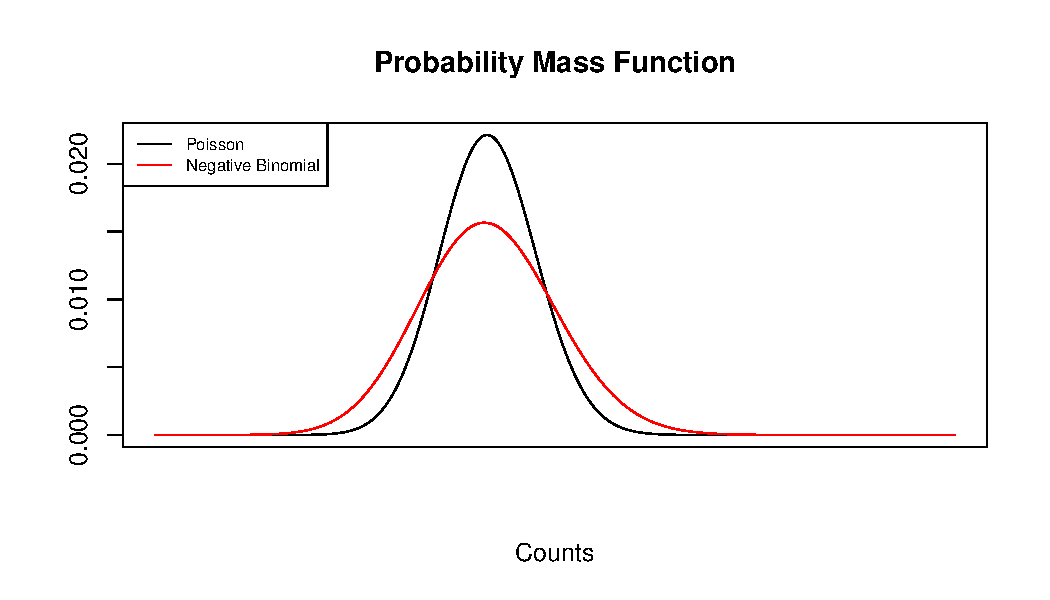
\includegraphics[width=\maxwidth]{figures/figunnamed-chunk-14-1} 
\end{knitrout}
\end{figure}

\end{frame}


\begin{frame}{Exact Methods vs MC simulations -- Gamma-Gamma Time}
\begin{figure}
\begin{knitrout}
\definecolor{shadecolor}{rgb}{0.969, 0.969, 0.969}\color{fgcolor}
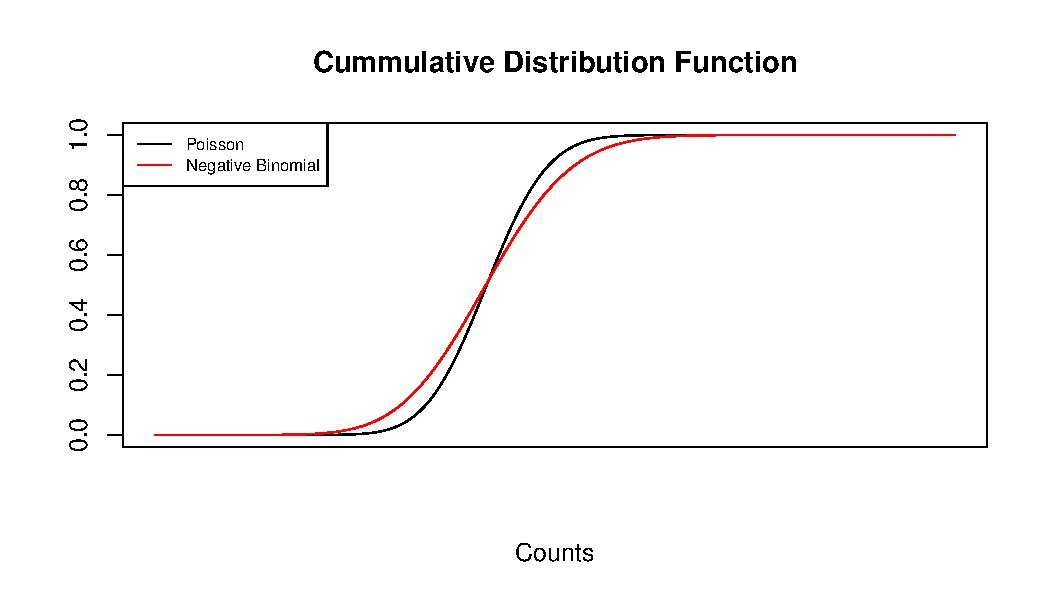
\includegraphics[width=\maxwidth]{figures/figunnamed-chunk-15-1} 
\end{knitrout}
\end{figure}
\end{frame}

\begin{frame}[shrink=20]{Exact Methods vs MC simulations}

\begin{table}[h!]
\centering
\begin{tabular}{cccc}
 \textbf{Model} & \textbf{Estimated Probabilty} & \textbf{MCse} & \textbf{Exact Probability} \\
\hline
\hline
 $C(T)\sim\textrm{Po}(\lambda T)$ & $\textrm{P}(C(T)\geq 324) = 0.5044$ & 0.005 & 0.5085 \\
 $C(T)\sim\textrm{PoG}(T, \alpha, \beta)$ & $\textrm{P}(C(T)\geq 324) = 0.4799$ & 0.005 & 0.5008 
\end{tabular}
\end{table}

\begin{table}[h!]
\centering
\begin{tabular}{cccc}
 \textbf{Model} & \textbf{Estimated Probabilty} & \textbf{MCse} & \textbf{Exact Probability} \\
\hline
\hline
 $T(C)\sim\textrm{G}(C, \lambda)$& $\textrm{P}(T(C)\geq 548) = 0.4978$ & 0.005 & 0.4955\\
$T(C)\sim\textrm{GG}(C, \alpha, \beta)$ & $\textrm{P}(T(C)\geq 548) = 0.5196$ & 0.005 & 0.5201
\end{tabular}
\end{table}
\textbf{Number of simulations:} $M=10^4$
\end{frame}

\begin{frame}{Aleatory VS Aleatory \& Epistemic}

\textbf{90\% chance} of accruing $Ctarget=324$ patients: 

\begin{itemize}
\item $M=10^3$ from Carter's $\rightarrow$ 580 days (innacurate)
\item Erlang exact distribution $\rightarrow$ 588 days
\item Gamma-Gamma exact distribution $\rightarrow$ 707 days
\end{itemize}
\end{frame}

\begin{frame}{Aleatory \& Epistemic}
\begin{figure}
\begin{knitrout}
\definecolor{shadecolor}{rgb}{0.969, 0.969, 0.969}\color{fgcolor}
\includegraphics[width=\maxwidth]{figures/figunnamed-chunk-16-1} 
\end{knitrout}
\end{figure}

\end{frame}

\begin{frame}{Conclusions}

\begin{itemize}
\item Visual tools
% Graphs clarify recruitment flow, delays, and patient leakage in trials
\item Unified Notation
% Consistent math framework allows precise analysis of count and time models
\item Exact Methods
% Extended Monte Carlo methods to capture both aleatory and epistemic uncertainty
\item Flexible Recruitment
% Framework supports both fixed and time-varying recruitment rates
\item Practical Impact
% Exact methods aid trial design; open-source R code enables real-world use
\end{itemize}
\end{frame}

% \begin{frame}{Summary}
% \begin{itemize}
% \item Exact distributions which extend Carter's approach
% \item Exact models for \textbf{counts} and their properties
% \item Unified notation
% \item Visualization of study accrual and uncertainty bands 
% \item Sensitivity analysis
% \end{itemize}
% 
% \end{frame}
% 
% 
% \begin{frame}{Next steps}
% \begin{itemize}
% \item Compare exact models for counts to those provided by \cite{carter2004application} based on MC simulations
% \item Models for \textbf{time} 
% 	\begin{itemize}
% 	\item Exact models
% 	\item Compare them to those provided by Carter
% 	\end{itemize}
% \item Apply theoretical results to dataset
% \item Shiny App
% \end{itemize}
% 
% \end{frame}

\begin{frame}{References}
  \small
  \bibliographystyle{apalike}
\bibliography{illustration}
\end{frame}


\begin{frame}{Thank you for your attention}

\end{frame}

%\appendix
%% Possible backup slides...

%% chapter division is accomplished with:
%% \part{Appendix}

\end{document}
